\chapter{Description et Conception des états}


\section{Description des états}

Dans un état du jeu, on retrouve des éléments fixes: les tiles (tuiles isometriques) qui composent la carte et des éléments mobiles: les personnages. Tous les éléments ont un nom et une position.

\subsection{Etat éléments fixes}

La carte du jeu est une table à 2 dimensions composée de tuiles.

Les tuiles sont générées de manière aléatoires. 
On retrouve dans les propriétés des tuiles : 
\\

\begin{itemize}
    \item \textbf{le type de tuile:} Il est critère de praticabilité pour un personnage et aussi pour l'affichage du sprite correspondant côté gestion rendu.
       \begin{itemize}
         \item[•]  Dirt
         \item[•]  Grass
         \item[•]  Water
         \item[•]  Sand
         \item[•]  Pound
         \item[•]  Rock
         \\
       \end{itemize}
    Les effets des types seront déterminés côté engine en fonction du type de tuile.
    \\
    \item \textbf{la hauteur:} Elle determine la hauteur de la tuile, modifieur impactant la distance de déplacement dans les actions et la portée d'une attaque qui seront gérés dans la partie engine. La hauteur est un entier compris entre 1 et 3.
\end{itemize}

\subsection{Etat éléments mobiles}

Les personnages appatiennent à des équipes. Chaque équipe est gérée par un joueur.  
Un personnage possède:
\\
\begin{itemize}
\item Une race générée aléatoirement parmi la liste suivante:
    \begin{itemize}
         \item[•]  Monster
         \item[•]  Beastman
         \item[•]  Demon
         \item[•]  Human
         \\
     \end{itemize}

\item Un job généré aléatoirement parmi la liste suivante:
    \begin{itemize}
         \item[•]  Pugilist
         \item[•]  Swordsman
         \item[•]  Archer
         \item[•]  Magician
         \\
     \end{itemize}
\item Un niveau calculé en fonction de l'expérience amassée.
\\ \\
Les caractéristiques (PV max, PM max, dégâts physiques, dégâts magiques, score d'évasion, score de défense, liste des compétences) sont déterminés en fonctions des 3 attributs précédents (race,job et niveau).
\\
\end{itemize}

Un curseur permet aux joueurs de navigueur sur les tuiles et lire les propriétés 
(du terrain et d'un personnage si présent) et sélectionner un personnage (si présent) en vue d'effectuer une action.


\subsection{Etat général}
En plus des éléments statiques et mobiles nous avons :
\begin{itemize}
         \item \textbf{nombre de tour:} Le nombre de tours qui ont été joués.
         \\
         \item \textbf{terminé:} Un booléen qui indique si le combat est terminé.
\end{itemize}

\section{Conception Logiciel}
Le diagramme des classes UML C++ pour les états est visible en Figure X. Nous pouvons mettre en évidence plusieurs groupes de classes qui sont les suivants :
\\
\begin{itemize}
    \item Groupe Character (bleu foncé): Toutes les charactéristiques des personnages, qu'ils soient ceux du joueur ou non, ainsi que les fonctions pour y accéder. Il présente une hiérarchie des classes filles permettant de visualiser les différentes catégories associées aux personnages et les types de chacun de ses élements.
    \\
    \item Groupe Team (bleu clair): Principalement composé de la classe Team, cette dernière englobe les ressources d'un joueur à savoir ses personnages et ses objets.
    \\
    \item Groupe Entity (jaune): La gestion du curseur et de l'entité pointée par ce dernier pour afficher les propriétés de la tuile à l'écran et selectionner le personnage qui réalise une action. 
    \\
    \item Groupe Observante (orange): Il sera implémenté en parallèle avec le render, pour pouvoir faire les tests.
    \\
    \item Groupe Turn (vert): Il représente l'état général durant un tour.
    \\
    \item Groupe Tile (gris): Ce groupe permet la construction d'une Tile aléatoire à l'aide de TileFactory. La carte sera formée à partir de ces Tiles. 
\end{itemize}

\section{Tests Unitaires}

Des tests unitaires ont été réalisés pour vérifier les fonctions des différentes classes. On réalise un fichier de test par classe.
Le code est couvert aux alentours de 88\% par les tests unitaires.

\newpage

\begin{figure}[H]
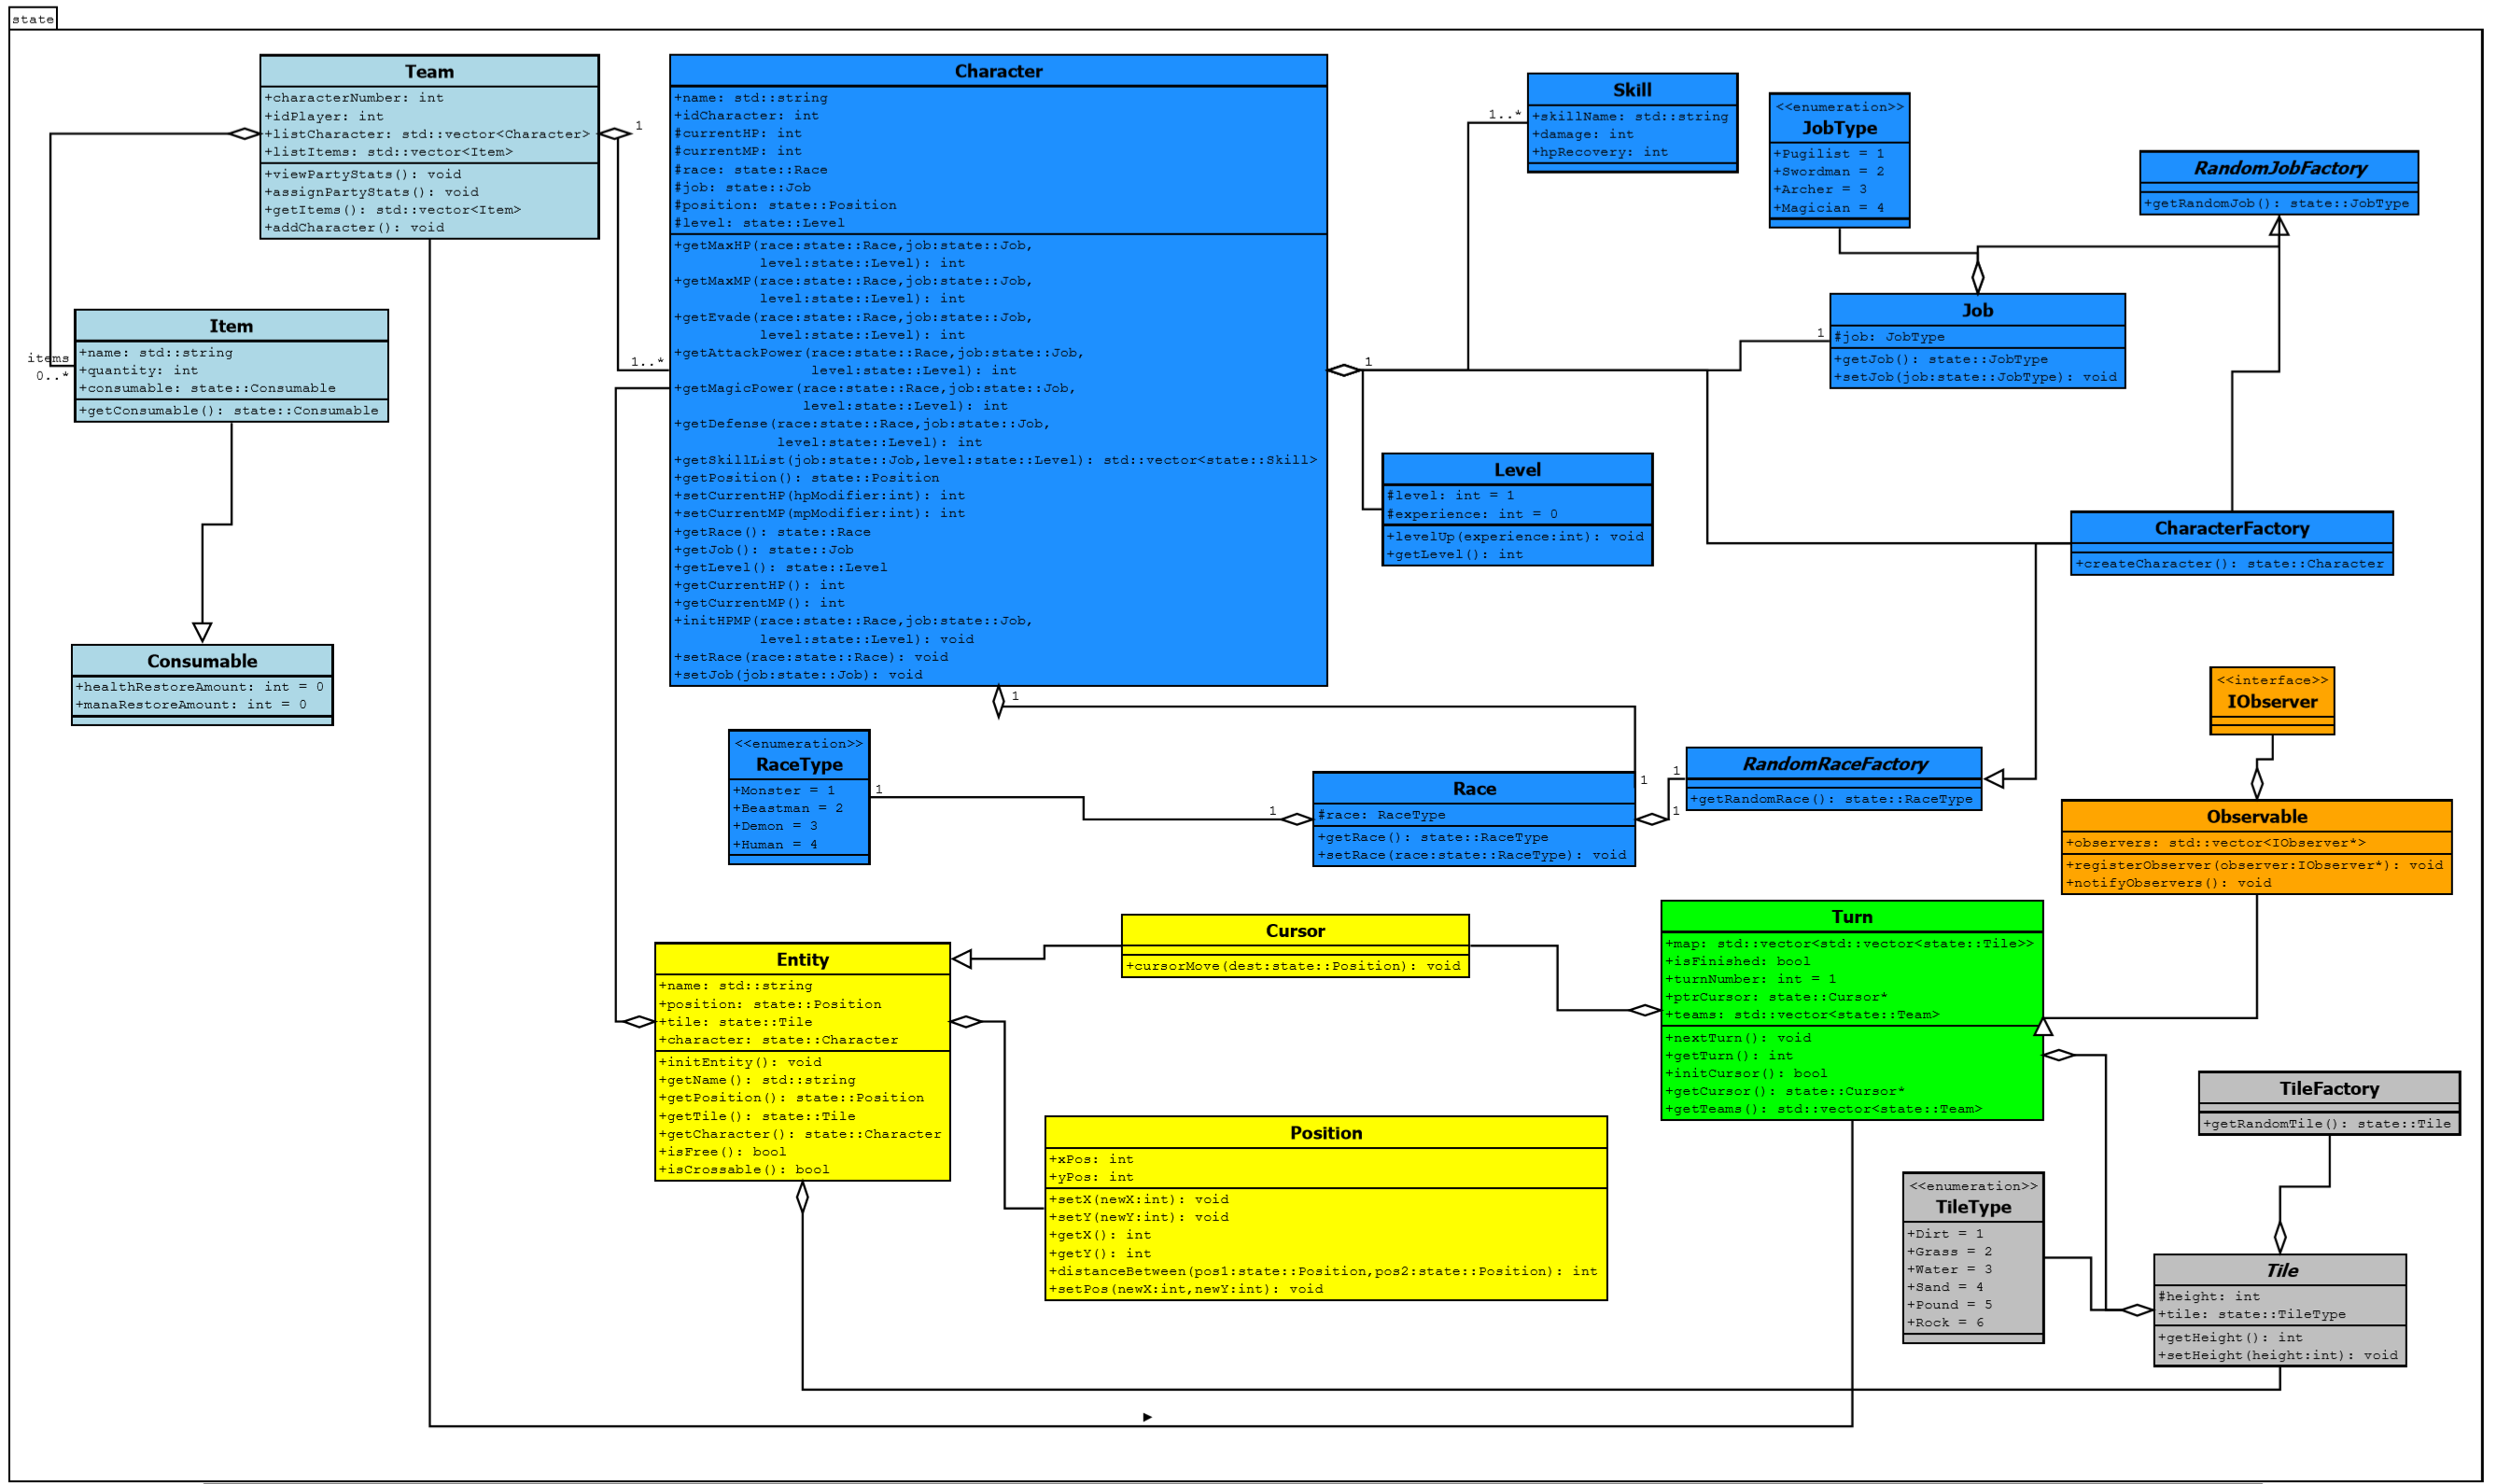
\includegraphics[width=\linewidth]{images/states.png}
\centering
\caption{Aperçu de state.dia}
\label{fig:img3}
\end{figure}
\newpage